Компьютерные вирусы представляют собой одну из наиболее серьёзных угроз информационной безопасности в современном мире. Ежедневно появляются десятки новых вредоносных программ, способных нанести значительный ущерб как отдельным пользователям, так и крупным организациям. Актуальность темы обусловлена необходимостью понимания природы компьютерных вирусов, механизмов их распространения и методов защиты от них.
 
\begin{figure}[h]
    \centering
    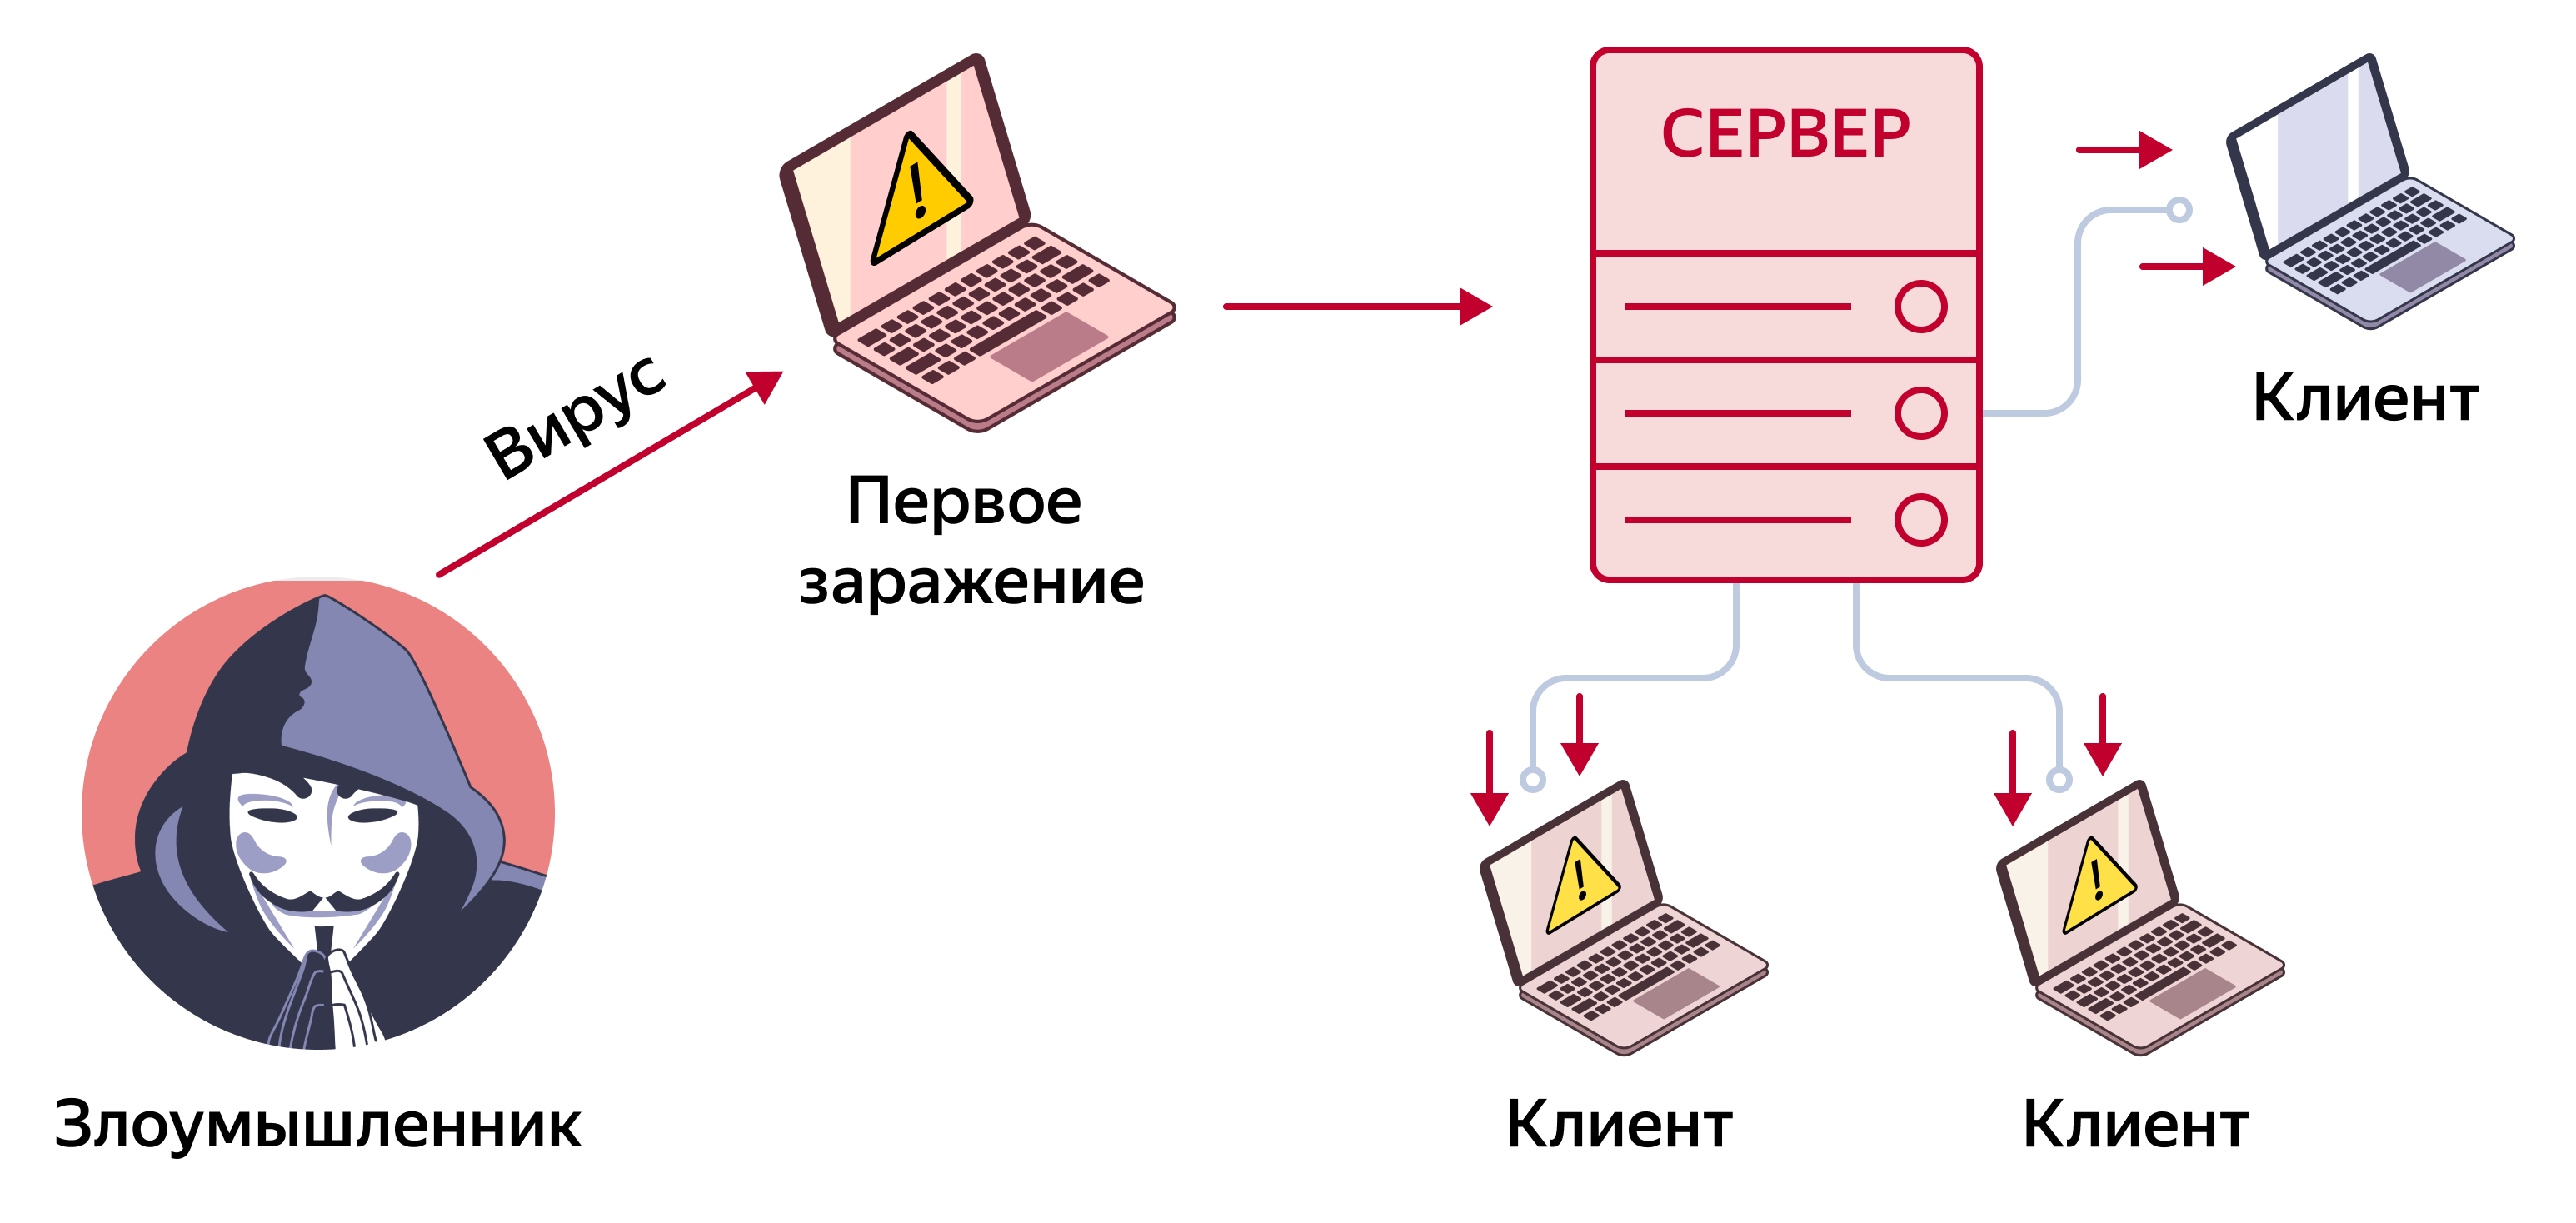
\includegraphics[width=0.5\textwidth]{images/virus_structure.png}
    \caption{Схематичное представление компьютерного вируса}
    \label{fig:virus_structure}
\end{figure}
 
\textbf{Цель} моего реферата --- изучить понятие компьютерного вируса, его классификацию, принципы работы и методы борьбы с ним.
 
Для реализации поставленной цели я ставлю перед собой следующие задачи:
 
\begin{enumerate}
    \item дать определение компьютерного вируса и рассмотреть историю их появления;
    \item изучить классификацию вирусов по различным признакам;
    \item разобрать механизмы работы вирусов на примере загрузочного вируса;
    \item рассмотреть признаки проявления вирусного заражения;
    \item изучить основные типы антивирусных программ и провести обзор современных антивирусных решений.
\end{enumerate}
 
\textbf{Объектом} исследования являются компьютерные вирусы как вредоносные программы, \textbf{предметом} исследования --- классификация вирусов и методы защиты от них.
 
В процессе работы над рефератом применялись анализ литературы, обобщение и систематизация информации.
 
Практическая значимость работы заключается в том, что её материалы могут быть использованы учащимися при изучении информационной безопасности, а также для выбора эффективных средств антивирусной защиты.